\documentclass[11pt]{article}

\usepackage{graphicx}
\usepackage[hidelinks]{hyperref}
\usepackage{appendix}
\usepackage{color, soul}
\usepackage{systeme}

\title{Software Engineering notes}
\author{Matteo Salvino}
\date{}

\begin{document}
\maketitle
\pagebreak
\tableofcontents
\pagebreak
\section{Capability Maturity Model Integration}
Now days companies want to deliver products and services better, faster and cheaper. At the same
time, in the high-technology environment of the twenty-first century, nearly all organizations have found themselves building increasingly complex products and services. It's unusual today for a single organization to develop all the components that compose a complex product or service. More commonly, some components are built in-house and some are acquired; then all the components are integrated into the final product or service. Organizations must be able to manage and control this complex development and maintenance process. The problems these organizations address today involve enterprise-wide solutions that require an integrated approach. Effective management of organizational assets is critical to business success. In other words, these organizations are product and service developers that need a way to manage their development activities as part of achieving their business objectives. In the current marketplace, maturity models, standard, methodologies and guidelines exist that can help an organization to improve the way it does business. However, most available improvement approaches focus on a specific part of the business and do not take a systematic approach to the problems that most organizations are facing. So, focusing on improving one particular business area, these models are hindered by barriers that exist in organizations. \textbf{CMMI} for development (CMMI-DEV) provides an opportunity to avoid or eliminate these barriers. It consists of best practices that address development activities applied to products and services. It address practices that cover the product's lifecycle from conception through delivery and maintenance. The goal is to build and maintain the total product. CMMI-DEV contains 22 process areas. Of those process areas, 16 are core process areas, 1 is a shared process area and 5 are development specific process areas. The Software Engineering Institute (SEI) in its research, has found some key points on which organizations can focus on to improve its business.
\begin{center}
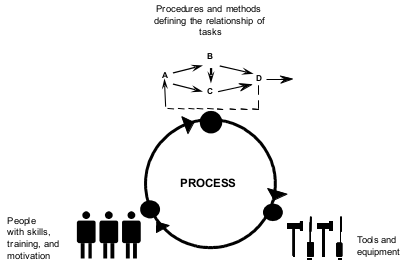
\includegraphics[scale=0.40]{./images/SEI_key_points.png}
\end{center}
In particular these key points are : people, procedures and methods, and tools and equipment. These points are kept together by the processes used in our organization. They allow us to address scalability and provide a way to incorporate knowledge of how to do things better. Processes allow us to leverage our resources and to examine business trends. We are focusing on methodologies, not because people and technologies aren't important, but since the technology changes at an incredible speed and people can works for different companies, in this way we can provides the infrastructure and stability necessary to deal with an ever-changing world and to maximize the productivity of people and the use of technology to be competitive. The SEI has taken the process management premise "the quality of a system of product is highly influenced by the quality of the process used to develop and maintain it" and defined CMMs that embody this premise. A CMM, including CMMI, is a simplified representation of the world, which contains the essential elements of effective processes. CMMs focus on improving processes in an organization, describing an evolutionary path from an immature process to disciplined mature process with improved quality and effectiveness. CMMI can be used in process improvements also as a framework, which provides the structure needed to produce CMMI models, training and evaluation components. To allow the use of multiple models withing the CMMI framework, model components are classified as either common to all CMMI models or applicable to a specific model. The common material is called \textbf{CMMI Model Foundation} (CMF). The components of the CMF are part of every model generated from the CMMI framework. Those components are combined with material applicable to an area of interest to produce a model. A \textbf{constellation} is defined as a collection of CMMI components that are used to construct models, training materials and evaluate related documents for an area of interest. CMMI-DEV previously introduced is the development constellation for a model. All CMMI models contains multiple \textbf{Process Areas} (PAs). A process area is a cluster of related practices in an area that, when implemented collectively, satisfies a set of goals considered important from making improvement in that area. Some of these area are : Causal Analysis and Resolution (CAR), Configuration Management (CM), etc. We can define two type of goal :
\begin{itemize}
\item \textbf{Generic} : it's called generic because the same goal statement applies to multiple process areas. A generic goal describes the characteristics that must be present to institutionalize processes that implement a process area. It's a required model component and is used in evaluation to determine whether a process area is satisfied or not. The istitutionalization is an important concept in process improvement, since it implies that the process in ingrained in the way the work is performed and there is a commitment and consistency to performing the process. The progress of process institutionalization is characterized by the type of the generic goal :
\begin{itemize}
\item \textbf{GG1 \- Performed process} : a performed process is a process that accomplishes the work necessary to satisfy the specific goals of a process area.
\item \textbf{GG2 \- Managed process} : a managed process is a performed process that is planned and executed in accordance with some policy. It employs skilled people having adequate resources to produce controlled outputs. It's controlled, monitored, reviewed and evaluated for adherence to its process description. The process can be instantiated by a project, group or organizational function. Management of the process is concerned with institutionalization and the achievement of other specific objectives established for the process, such as cost, schedule and quality objectives. The control provided by a managed process helps to ensure that the established process is retained during times of stress. The requirements and objectives for the process are established by the organization. The status of the work products and services are visible to management at defined points. Commitments are established among those who perform the work and the relevant stakeholders and are revised as necessary. Work products are reviewed with relevant stakeholders and are controlled. A critical distinction between a performed process and a managed process is the extent to which the process is managed. A managed process is planned and its execution is managed against the plan. Corrective actions are taken when the actual results and execution deviate significantly from the plan. A managed process achieves the objectives of the plan and is institutionalized for consistent execution. 
\item \textbf{GG3 \- Defined process} : a defined process is a managed process that is tailored from the organization's set of standard processes according to the organization's tailoring guidelines. It has a maintained process description and contributes process related experiences to the organizational process assets. Organizational process assets are artifacts that relate to describing, implementing and improving processes. These artifacts are assets because they are developed or acquired to meet the business objectives of the organization and they represent investments by the organization that are expected to provide current and future business value. The organization's set of standard processes, which are the basis of the defined process, are established and improved over time. Standard processes describe the fundamental process elements that are expected in the defined processes. Standard processes also describe the relationships among these process elements. A project's defined process provides a basis for planning, performing and improving the project's task and activities. A critical distinction between a managed process and a defined process is the scope of application of the process descriptions, standards and procedures. For a managed process, the process descriptions, standards and procedures are applicable to a a particular project, group or organizational function. As a result, the managed processes of two projects in one organization can be different. Another critical distinction is that a defined process is described in more detail and is performed more rigorously than a managed process. Finally, management of the defined process is based on the additional insight provided by an understanding of the interrelationships of the process activities and detailed measures of the process, its work products, and its services.
\end{itemize}
\item \textbf{Specific} : a specific goal describe the unique characteristics that must be present to satisfy the process area. It's a required model component and is used in evaluation to determine whether a process area is satisfied or not.
\end{itemize}
\subsection{Understanding levels}
Levels are used in CMMI-DEV to describe an evolutionary path recommended for an organization that wants to improve the processes it uses to develop products or services. CMMI supports two improvement paths using levels. One path enables organizations to incrementally improve processes corresponding to an individual process area selected by the organization. The other path enables organizations to improve a set of related processes by incrementally addressing successive sets of process areas. These two improvement paths are associated with the two types of levels : \textbf{capability levels} and \textbf{maturity levels}. These levels correspond to two approaches to process improvement called \textbf{representations}. In turn, the two representations are called \textbf{continuous} and \textbf{staged}. Both representations provide ways to improve our processes to achieve business objective and use the same model components. The continuous representation is concerned with selecting both a particular process area to improve and the desired capability level for that process area. The staged representation is concerned with selecting multiple process areas to improve within a maturity level. Both capability levels and maturity levels provide a way to improve the processes of an organization and measure how well organizations can and do improve their processes. However, the associated approach to process improvement is different.
\subsubsection{Capability levels (Continuous representation)}
To support those who use the continuous representation, all CMMI models reflect capability levels in their design and content. The four capability levels, each of them is a layer for the process improvement, are designated by the numbers 0 through 3 :
\begin{itemize}
\item \textbf{0. Incomplete} : an incomplete process is a process that either is not performed or is partially performed. One or more of the specific goals of the process area are not satisfied and no generic goals exist for this level since there is no reason to institutionalize a partially performed process.
\item \textbf{1. Performed} : a performed process is a process that accomplish the needed work to produce work products; the specific goals of the process area are satisfied.
\item \textbf{2. Managed} : a managed process is a performed process that is planned and executed in accordance with some policy; It employs skilled people having adequate resource to produce controlled outputs; it involves relevant stakeholders; It's monitored, controlled, reviewed and evaluated for adherence to its process description. The process discipline reflected by capability level 2 helps to ensure that existing practices are retained during times of stress.
\item \textbf{3. Defined} : a defined process is a managed process that is tailored from the organization's set of standard processes according to the organization's tailoring guidelines and contributes work products, measures, and other process improvement information to the organizational process assets.
\end{itemize}
\subsubsection{Maturity levels (Staged representation)}
To support those who use the staged representation, all CMMI models reflect maturity levels in their design and content. A maturity level is a defined evolutionary plateau for organizational process improvement. Each maturity level matures an important subset of the organization's processes, preparing it to move to the next maturity level. The maturity levels are measured by the achievement of the specific and generic goals associated with each predefined set of process areas. The five maturity levels are designated by the numbers 1 through 5 :
\begin{itemize}
\item \textbf{1. Initial} : in this layer processes are usually ad hoc and chaotic. In spite of this chaos, maturity level 1 organizations often produce products and services that work, but they frequently exceed the budget and schedule documented in their plans. These organizations are characterized by a tendency to overcommit, abandon their processes in a time of crisis, and be unable to repeat their successes.
\item \textbf{2. Managed} : as before.
\item \textbf{3. Defined} : as before.
\item \textbf{4. Quantitatively managed} : it's a defined process that is controlled using statistical and other quantitative techniques. Quantitative objectives for quality and process performance are established and used as criteria in managing the process. Quality and process performance is understood in statistical terms and is managed throughout the life of the process.
\item \textbf{5. Optimizing} : it's a quantitatively managed process that is improved based on understanding of the common causes of variation inherent in the process. The focus of an optimizing process is on continually improving the range of process performance through both incremental and innovative improvements.
\end{itemize}
\subsection{ISO family}
\textbf{ISO 12207} defines and structures all activities involved in the software development process. Its main goal is to provide a common language to involved stakeholders. It's based on a functional approach : a set of coordinated activities transforming an input in an output. It's based on two basic principles :
\begin{itemize}
\item \textbf{Modularity} : it means processes with minimum coupling and maximum cohesion.
\item \textbf{Responsibility} : it means to establish a responsibility for each process, in order to facilitate the application of the standards in a project where there are many people involved.
\end{itemize}
\textbf{ISO 9000} is maintained by ISO and is administered by accreditation and certification bodies. This family of ISO addresses "Quality management". Its fundamental building blocks are :
\begin{itemize}
\item \textbf{Quality management system} : it deals with general and documentation requirements that are the foundation of the management system. In particular, the previous requirements can be explained in details :
\begin{itemize}
\item \textbf{General} : they are general requirements like how the processes of the management system interact to each other or how you will measure and monitor the processes.
\item \textbf{For documentation} : they are requirement focused on the documentation. They can require what documentation is needed to operate the system effectively or how it should be controlled.
\end{itemize}
\item \textbf{Management responsibility} : it manage high level responsibilities like set policies and objectives or plan how the objectives will be met.
\item \textbf{Resource management} : it deals with the people and physical resources needed to carry out the process. People should be competent to carry out their task and physical resources and work environment need to be capable of ensuring that the customer's requirements are satisfied.
\item \textbf{Product-service realization} : it deals with the processes necessary to produce the product or to provide the service.
\item \textbf{Measurement, analysis, and improvement} : it deals with measurements to enable the system to be monitored. For example we can measure if the processes are effective or if the product really satisfy customer's requirements.
\end{itemize}
ISO doesn't itself certify organizations. There are accreditation bodies that authorize certification bodies. Organizations can apply for ISO 9001 compliance certification to a certification body. The various accreditation bodies have mutual agreements with each other to ensure that certificates issued by one of the Accredited Certification Bodies (CB) are accepted worldwide. An ISO certificate is not a once-and-for-all award, but must be renewed at regular intervals recommended by the certification body, usually around three years. \textbf{Quality requirements} are a set of process requirements and resources that constitute the Quality Manual (QM) of the organization. This latter specifies the organization's quality policy regardless specific commitments and customers. It's adapted to specific projects, generating several Quality Policies (QP). The ISO 9001 certification required that processes are described in the two previous specific documents (QM and QP).
\section{Software Development Process Models}
Software products are not tangible. In order to manage a software project the project manager needs special methods. So, the monitoring process in based on the explicit definition of activities to be performed and documents to be produced. These documents allow us to monitor the progress of the process and give us an idea of its quality. Software Development Process Models and their instances, differ from each other for the required activities and for the produced documents. Now, we will see several software process models, discussing their pros and cons.
\subsection{Waterfall model}
A Waterfall model is a typical process in which there are separate and distinct phases of specification and development. So, first we describe all the specifications of the software and then we have a subsequent phase that take care about the development. Its main phases are :
\begin{itemize}
\item \textbf{Requirements analysis and definition}
\item \textbf{System and software design}
\item \textbf{Implementation and unit testing}
\item \textbf{Integration and system testing}
\item \textbf{Operation and maintenance}.
\end{itemize}
Each phase depends on the deliverables of the previous one and corresponds to a specialization of tasks. One of its main drawback is the difficulty of allows changes after the process in started. Another drawback is that the end users doesn't have a vision of the overall system (uncertainty). So, they have to wait till a working version of the system is available. In turn, programmers have to wait the analysis phase before starting their job. The solution is to use an iterative approach.
\subsection{Process iteration}
The system requirements always evolve during the project development, so process iteration where earlier stages are reworked is always part of the process for large systems. Iteration can be applied to any of the generic process models. Typically, an iteration follows one of the following approaches :
\begin{itemize}
\item \textbf{Incremental delivery} : we start building a small system (prototype) and next we enlarge it (incremental way). A \textbf{prototypal model} is constituted by a customer interaction in order to obtain customer's requirements, then we build a prototype also called \textbf{mock-up}  (when we build a system with feels and looks similar to the final system, but without working software behind), and then we present it to the user, in order that he is able to test the prototype and say "Ok, i'm satisfied", or viceversa. If the answer is positive, then we can start to implement the functionality behind the mockup. The \textbf{incremental model} is formed by iterations which are constituted by analysis, design, implementation and test phases. The result of a generic iteration $i$ typically is the system with version $i$. It's very similar to the prototypal model but in this case the intermediate version are full working and it allows for a more accurate design. Its main drawback is that if we figure out a wrong functionality in a specific system version, we have to throw away a lot of job previously done, whereas in the first model we will build only the mock-up system. In the incremental development we define the requirements, then we assign each of them to a specific system release version, design the whole system architecture, then develop, validate and integrate the system increment, and finally validate the system. If this isn't the last iteration, then we continue to increment the functionality of our system, otherwise we have built the final system. In other words, delivering part of the required functionality. Then the user requirements are prioritized and the highest priority requirements are included in early increments (early versions). Once the development of an increment is started, the requirements are frozen though requirements for later increments can continue to evolve. The trade off is the length of these iterations, the bigger the interval is then we move towards the waterfall model, the smaller the interval is then will be more difficult to build a very good software architecture. Its advantages are the following : the customer can see at each iteration an increment of the system functionalities, early increments act as a prototype to help asking requirement for future iterations, lower risk of overall project failure and the highest priority system requirements tends to receive the most testing.
\item \textbf{Spiral development} : in spiral development the process is represented as spiral (rather than a sequence) of activities. Each loop in the spiral represents a phase in the process. There not exist fixed phases such as specification or design (the loops in the spiral are chosen depending on what is required). The risks are explicitly evaluated and resolved throughout the process. In particular, the spiral model is constituted by the following sectors :
\begin{itemize}
\item \textbf{Objective setting} : they are specific objectives for the current phase.
\item \textbf{Risk assessment and reduction} : the risks are evaluated and activities punt in place to reduce the key risks.
\item \textbf{Development and validation} : in this sector we choose a development model for the system.
\item \textbf{Planning} : the project is reviewed and the next phase of the spiral is planned.
\end{itemize}
\end{itemize}
\subsection{Formal methods}
Formal methods are formalisms based on logic or algebra for requirement specification, development and test. They don't use the natural language, because it's very ambiguous, but tends to write the specification of the software in some formal languages like Z, Z++, etc.
\subsection{Extreme programming}
It's a part of the Agile model family. It's an approach based on the development and delivery of very small increments of functionality. It relies on constant code improvement, use involvement in the development team and pairwise programming.
\subsection{Core process activities}
Now, lets quickly review the main activities involved in the development process :
\begin{itemize}
\item \textbf{Software specification} : it's the process of establishing what services are required and the constraints on the system operations and development. These requirements can be functional or non-functional (they regards about system quality). This process is also called requirements engineering process. First of all it perform a feasibility study to understand if building the system is feasible. Typically this phase produce a document called feasibility report. Subsequently, the requirements are defined, analyzed and validated. The results of these phases constitute the so called requirement document.
\item \textbf{Software design and implementation} : it's the process of converting the system specification into an executable system. The software design phase is a process that in which we design the software structure (architectural, component, data structures, etc.) that fulfill the specifications. In the implementation phase we translate the previous structure into an executable program. In this phase our goal is also to remove as many errors as possible from the program generated, typically using a program testing. These two phases are closely related and may be interleaved. 
\item \textbf{Software validation} : the verification and validation is intended to show that the system is conform to its specifications (verification) and meets the customer's requirements (validation). Typically the system is tested over test cases that are derived from the specification of the real data to be processed by the system. We can use several types of testing :
\begin{itemize}
\item \textbf{Unit test} : individual components are tested independently.
\item \textbf{System test} : test the whole system.
\item \textbf{Acceptance test} : testing with customer data to check that the system meets the customer's needs.
\end{itemize}
\item \textbf{Software evolution} : software is very flexible and can change over time. A change of the requirements must be reflected also in the software.
\end{itemize}
\section{Scrum}
Scrum is an agile process that allows us to focus on delivering the highest business value in the shortest time. It allows us to rapidly and repeatedly inspect actual working software (every two week to one month). The business set the priorities. Team self-organize to determine the best way to deliver the highest priority features. Every two weeks to a month anyone can see real working software and decide to release it as is or continue to enhance it for another sprint. The requirements of the customer are captured as items in a list of "product backlog". The core values of Scrum are the following :
\begin{itemize}
\item \textbf{Commitment} : teams commit to their goals for the sprint, product owners commit to ordering the product backlog and ScrumMasters commit to removing any obstacles along the way in order to simplify the flow of product development. The Scrum team should do whatever is necessary in order to meet their goals, and it's important that they are empowered to do so.
\item \textbf{Focus} : for a team to be able to complete its work, its members must be allowed to focus. The ScrumMaster doesn't allow changes in the sprint's commitment so that the team may keep its focus. When a team gives its full attention to the problem, its work is much more productive, predictable and fulfilling.
\item \textbf{Openness} : as Scrum uses empirical process control to make progress through a project, it's essential that the results and experience of an experiment (i.e. a sprint) are visible. Once visibility exists, inspection and adaption can occur.
\item \textbf{Respect} : in order to be its best, a team's members need to respect for each other and, the knowledge that each brings to the table, experiences, working styles and personalities. Respect doesn't come for free, it's earned. Scrum team members should be dedicated, cross-functional, empowered and self-organizing.
\item \textbf{Courage} : it takes buckets of courage for a ScrumMaster to apply Scrum the way it was intended. One of the primary responsibilities of the ScrumMaster is to help the organization identify its weaknesses so that it may improve. This takes courage. Sometimes, a team has to push back on the product owner when asked to take on too much during a sprint. It takes courage to say no to that sort of pressure. A product owner must have courage when communicating with other stakeholders about the reality of a project. 
\end{itemize}
\subsection{Roles}
\paragraph{Scrum team} The Scrum team includes the product owner, ScrumMaster and the team members, whereas the Scrum delivery team is a subset made of only the technical team members. The whole Scrum team huddles around a problem (i.e. a requirement from the Product Backlog) and innovates solutions. Scrum teams should be five to nine team members, dedicated to the life of the project, cross-functional, empowered and self-organizing. Scrum teams plan, estimate and commit to their work, rather than a manager performing these activities for them. The end goal of the team is to deliver a potentially shippable product increment that meets an agreed-upon Definition of Done each and every sprint.
\paragraph{Product owner} The product owner is responsible for the product's success. In other words, while the team is responsible for delivering a quality solution, the product owner is responsible for knowing his market and user needs well enough to guide the team towards a marketable release sprint after sprint. In a project there should be one and only one product owner who makes final decisions about the direction of the product and the order in which features should be developed. The product owner, since he is represent the "what" and "why" of the system, should be available to the team to have regular dialog about the requirements in the product backlog; additionally, the product owner must make the product vision clear to everyone on the team and regularly maintain the product backlog in keeping with the product vision. The product owner always keeps the next set of product backlog items in a ready state so that the team always has work in the queue for the next sprint.
\paragraph{ScrumMaster} The ScrumMaster safeguards the process. He/she understands the reasons behind and for an empirical process, and does his or her best to keep product development flowing as smoothly as possible. This leader protects team members from interruptions in order to keep them focused on their sprint commitments. The ScrumMaster also facilitate all Scrum meetings, ensuring that everyone on the team understands the goals and that they share a commitment together as a true team and not just as a collection of individuals. She/he removes obstacles that prevent a steady flow of high-value features.
\subsection{Ceremonies}
A sprint is an iteration defined by a fixed start and end data; it's kicked off by sprint planning and concluded by the sprint review and retrospective. The team meets daily, in a daily scrum meeting, to make their work visible to each other and synchronize based on what they've learned. Lets discuss in details these phases one at a time.
\paragraph{Sprint planning} During sprint planning the product owner and the team discuss the highest priority items in the product backlog and brainstorm a plan to implement those items. The set of chosen product backlog items and their subsequent tasks collectively is referred to as the team's sprint backlog. The sprint planning meeting is time-boxed to eight hours for a 30-day sprint, reduced proportionally for shorter sprints. The meeting is constituted by two parts : the first one is driven by the product owner who presents the most important product backlog items (with the support of drawings, mockups, etc.) and clarifies question from the development team about what he/she wants and why he/she wants it. The second part is driven by the Scrum delivery team who work together to brainstorm approach and eventually agree on a plan. It's at the start of this second part that the sprint actually begins. Of course, teams are always searching for ways to make planning faster and more efficient. The result of sprint planning is a sprint backlog that is comprised of selected product backlog items for the sprint, along with the correlating tasks identified by the team in the second part of sprint planning.
\paragraph{Sprint review} The sprint review provides the opportunity for stakeholders to give feedback about the emerging product in a collaborative setting. In this meeting, the team, product owner, ScrumMaster and any interested stakeholders meet to review and talk about how the product is shaping up, which features may need to change and perhaps discuss new ideas to add to the product backlog. It's common for a ScrumMaster to summarize the event of the sprint, any major obstacles that the team ran into, and so on, and of course the team should always demo what they've accomplished by the sprint's end. This meeting is time-boxed to four hours for a 30-day sprint.
\paragraph{Sprint retrospective} During the final spring meeting, the sprint retrospective, team members discuss events of the sprint, identify what worked well for them, what didn't work so well and take on action items for any changes that they would like to make for the next sprint. The ScrumMaster will take on any actions that the team doesn't feel it can handle. The ScrumMaster reports progress to the team regarding these obstacles in subsequent sprints. This meeting is time-boxed to three hours.
\paragraph{Daily scrum meeting} In the daily scrum meeting team members make their progress visible so that they can inspect and adapt toward meeting their goals. The meeting is held at the same time and in the same place, decided upon by the team. Even  though a team makes its best attempt at planning for a sprint, things can change in flight. In this 15-minute meeting, team members discuss what they did since yesterday's meeting, what they plan to do by tomorrow's meeting, and to mention any obstacles that may be in their way. The ScrumMaster record any obstacles that the team members feel they cannot fix for themselves and will attempt to remove them after the meeting. The scrum delivery team members, product owner and ScrumMaster are participants in the meeting. Anyone else is welcome to attend but only as observers.
\subsection{Artifacts}
\paragraph{Product backlog} The product backlog is the product owner's "wish list". Anything and everything that they think they might want in the product goes in this list. The product owner maintains the product backlog, although other stakeholders should have visibility of and the ability to suggest new items for the list. The product owner prioritizes the product backlog, listing the most important or most valuable items first. Once a team selects items for a sprint, those items and their priorities are locked; however, priorities and details for any not-started work may change at any time. Through this mechanism, teams are able to focus on this sprint's work while the product owner retains maximum flexibility in ordering the next sprint's work.
\paragraph{Sprint backlog} Owned by the team, the sprint backlog reflects the product backlog items that the team committed to in sprint planning, as well as the subsequent tasks and reminders. Team members update it every day to reflect how many hours remain on his/her task; team members may also remove tasks, add tasks or change tasks as the sprint is started.
\paragraph{Product increment} The product increment is a set of features, user stories or other deliverables completed by the team in the sprint. It should be potentially shippable (i.e. it must have enough quality to give it to the users). The product owner is responsible for accepting the product increment during each sprint, according to the agreed-upon Definition of Done and acceptance criteria for each sprint deliverable. Without a product increment, the product owner and other stakeholders have no way to inspect and adapt the product. A team must keep its progress visible at all times. It will create many additional artifacts in order to ensure visibility. Some common visibility tools are the release and sprint burndown charts. A burndown chart display of what work has been completed and what is left to complete. It is provided for each developer or work item. It's updated every day and make best guess about hours/points completed each day. A possible variation of this chart is called release burndown chart, which display how much work remain in the release backlog at the end each sprint (it shows overall progress).
\section{Layers vs Tiers}
Typically an information system is constituted by three layers : presentation, application logic and resource management layer. The \textbf{presentation layer} is devoted to present the system's user interface to clients. The \textbf{application logic} determines what the system actually does. It takes care of enforcing business processes. The application logic can take many forms : programs, constraints, etc. The \textbf{resource manager} deals with the organization (storage, indexing and retrieval) of the data necessary to support the application logic. This is typically a database but it can also be a text retrieval system or any other data management system providing querying capabilities and persistence. A client is any user or program that wants to perform an operation over the information system. Clients are independent of each other : one could have several presentation layers depending on what each client wants to do. One can take advantage of the computing power at the client machine to have more sophisticated presentation layers. This also saves computer resources at the server machine. It introduces the concept of API, an interface to invoke the system from the outside. It also allow designers to think about federating the systems into a single system. The resource manager only sees one client : the application logic. This improve a lot the performance since there aren't client connections/session to maintain. A \textbf{tier} is a physical level. How can we divide logical layers over physical objects ? The first architecture developed is the so called \textbf{1-tier architecture}, in which all layers are running on the same machine (i.e. a mainframe). The second approach is called \textbf{2-tier architecture}, in which we can have one machine (server) that contains the application logic and resource management and another one (client) that contains the presentation layer. This approach is also called client-server architecture. The evolution of this concept is to introduce micro services, and using a \textbf{3-tier architecture}, in which the presentation layer runs on the client machine, the application logic layer on a middle machine and the resource management layer on a dedicated machine. The problem is that now, we have more connections respect to the previous architectures. In fact, the middle's developers needs to write the code for  receiving requests from the client and from the server. So, the people realize that needed something more, a specific technologies called \textbf{middleware}, that could make the development of the code as much simple as if the code is still running in the mainframe (on the same machine). Once you know how to split the software in three layers, you can split each of them in more layers on its own machine, in order to make load balance. The result of this idea is called \textbf{N-tier architecture}.
\subsection{Middleware}
A middleware can serves the requests in two ways :
\begin{itemize}
\item \textbf{Synchronous} : traditionally, distributed applications use blocking calls, in which the client sends a request to a service and waits for a response of the service to come back before continuing doing its work. This type of interaction require both parties to be online : the client make the request, the receiver gets the request, processes it and sends a response to the caller, the client receives the response. Due it synchronizes client and server, this approach has several disadvantages : 
\begin{itemize}
\item \textbf{connection overhead} : synchronous invocations require to maintain a session between the caller and the receiver. Maintaining a session is expensive and consumes CPU resources. There is also a limit on the number of session that can be active at the same time. For this reason, client/server systems often use connection pooling (pooling of connections, with a thread associate at each of them and allocate one of them when needed) to optimize resource utilization. Synchronous interaction requires a context for each call and a context management system for all incoming calls. The context needs to be passed around with each call as it identifies the session, the client and the nature of the interaction.
\item \textbf{higher probability of failures} : if the client or the server for some reason fail, the context is lost and resynchronization is difficult. Finding out when the failure took place may not be easy.
\end{itemize}
To the previous problems there are two solutions :
\begin{itemize}
\item \textbf{Enhanced support} : we can use transactional interaction to enforce exactly once execution semantics and enable more complex interactions with some executions guarantees. Another approach is service replication and load balancing, in order to prevent the service from becoming unavailable when there is a failure.
\item \textbf{Asynchronous interaction} : see below.
\end{itemize}
\item \textbf{Asynchronous} : using asynchronous interaction, the caller sends a message that gets stored somewhere until the receiver reads it and sends a response. The response is sent in a similar manner as before. This type of interaction can take place in two forms :
\begin{itemize}
\item \textbf{non-blocking invocation} : a service invocation but the call returns immediately without waiting for a response, similar to batch jobs.
\item \textbf{persistent queue} : the call and the response are actually persistently stored until they are accessed by the client and the server.
\end{itemize}
\end{itemize}
A middleware can be implemented with two approaches :
\begin{itemize}
\item \textbf{Programming abstraction} : it's an approach intended to hide low level details of hardware, network and distribution. Middleware is primarily a set of programming abstractions developed to facilitate the development of complex distributed systems; to understands a middleware platform one needs to understand its programming model. From this latter can be determined its limitations, general performance and applicability of a given type of middleware. Furthermore, this model also determines how the platform will evolve.
\item \textbf{Infrastructure} : as the programming abstraction reach higher and higher levels, also the infrastructure that implements the abstractions must grow accordingly. Additional functionality is always implemented through additional software layer. The additional software layers increase the size and the complexity of the infrastructure necessary to use the new abstractions. The infrastructure is also intended to support additional functionality that makes development, maintenance and monitoring easier and less costly. It takes care of all non-functional properties typically ignored by programming models and languages such as performance, maintenance, resource management, etc.
\end{itemize}
Typically a middleware is based on RPC, in which the client invoke a local procedure talking with its stub (client stub), which is able to communicate with the remote object via a communication module. A request is created putting the client parameters, serialized (marshal operation) and send to the server stub. The server dispatcher deliver the serialized request to its stub, which deserialize (unmarshal operation) it, extract the parameters and finally call the server procedure. When there are more entities interacting with each other, RPC treats the calls as independent of each other. The main drawback of RPC is that recovering from partial system failures may be very complex. So, a programmer instead to implement the whole infrastructure for a distributed application can use an RPC system, which hides distribution behind procedure calls, provides an interface definition language (IDL) to describe the services, generates all the additional code necessary to make a procedure call remote and to deal with all the communication aspects and provides a binder in case it has a distributed name and directory service system. The solution to this limitation is to make RPC calls transactional, i.e. instead of providing plain RPC, the system should provide TRPC. It's based on the same concepts of RPC but, use additional language constructs and runtime support to bundle several RPC calls into an atomic unit.
\subsubsection{Message Oriented Middleware}
MOM is software or hardware infrastructure supporting sending and receiving messages between distributed systems, with the following structure :
\begin{center}
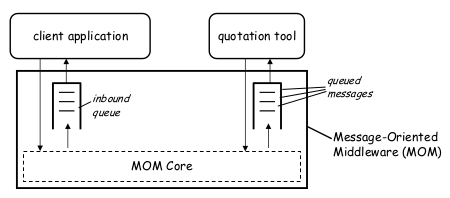
\includegraphics[scale=0.55]{./images/MOM_schema.png}
\end{center}
The participants of the communication are divided into two groups :
\begin{itemize}
\item \textbf{Publisher} : the entity that send messages
\item \textbf{Subscriber} : the entity that express interest in certain categories of messages.
\end{itemize}
The main disadvantage of this approach is that require an extra component in the architecture called \textbf{event service} that receives messages from publisher and cross-check them with the interests of subscribers. As with any system, an introduction of another component can lead to performance and reliability reduction, and can make the whole system more difficult and expensive to maintain. The information can be processed in two ways :
\begin{itemize}
\item \textbf{Topic-based} : the publisher is responsible for defining the topics to which subscribers can subscribe.
\item \textbf{Content-based} : filters can be used for a more accurate selection of information to be received.
\end{itemize}
The publisher can specify which topics are available for a subscription (topic-based) and subscribers can specify particular attribute in order to filtering the messages of interest. 
The notification can be made in two ways :
\begin{itemize}
\item \textbf{push} : the subscribers are invoked in callback, using a reference communicated at the time of subscription.
\item \textbf{pull} : the subscribers poll the event service when they need messages.
\end{itemize}
\hl{To-Do : add the pseudocode !}
\section{Web Services}
Web services are the current evolution of middleware technology. Basically are offered in a way over Internet. In other words, a web service is a software functionality exposed over the Internet. This means that any piece of code and any application component deployed on a system can be transformed into a network-available service. The main difference between middleware and web services, is Internet, because the latter emerged at the beginning of 2000 (when vendors invented new technologies and standard). So, web services perform business functions such as :
\begin{itemize}
\item a self-contained business task (for example a funds deposit service)
\item the whole business process (for example the automated purchasing of office supplies)
\item an entire application (for example demand forecasts and stock replenishment)
\item a service-enable resource (for example access to a particular back-end database containing some interesting data).
\end{itemize}
Once we have these functionalities exposed over Internet we can mix and match them to create a complete process. Until the emergence of web service technology the client and server should be on the same web platform (OS or programming language). With web service we can use whatever programming language and operating system that talks each other (i.e. platform independent). When we develop a web service we need to take into account the billing model, i.e. the mode in which the customer can pay in order to use specific functionalities of the service exposed. An \textbf{Application Service Providers (ASP)} is based on the idea to rent its own applications to subscribers such that :
\begin{itemize}
\item the whole application is developed in terms of user interface, workflow, business and data components that are all bound together to provide a working solution.
\item an ASP hosts the entire application and the customer has little opportunity to customize it beyond the appearance of the user interface.
\item an alternative of this is where the ASP is providing a software module that is downloaded to the customer's site on demand (situations in which the software can operate remotely via a browser).
\end{itemize}
When we have an ASP model it offers the whole application suite to the customers, which introduce the concept of software-as-a-service (i.e. pay for the application but we don't own it). This approach has several limitations such as : inability to develop high interactive applications, inability to provide complete customizable application and inability to integrate applications. With Web Services is different because we aren't paying for the whole application, but many different providers offers the functionalities that are needed for someone to develop the software. This is the key difference between ASP and Web Service approach. When we have an ASP, it is able to complete a full fledged application, and then the customer can exploit the application viewing it in the browser. When we have Software-as-a-Service, we have an entire application deployed by the service provider, and this software is downloaded on demand on the customer site and he performs its executed software on his side without accessing a browser. When we have a web service, the idea is that the ASPs offers basic components and then the customer can compose them in order to run on his premise or to have another ASP that composes the services offered by third party. A question to ask ourselves is where are services used ? Typically we have two types of usage :
\begin{itemize}
\item \textbf{within an enterprise} : web services are intended for being used for enterprise application integration. In this case, they are used to improve the reuse, reduce the skill requirements, can save on infrastructure, deployment and management costs, since we have these components already packed, and can accelerate and reduce the cost of integration as creating new application is simpler than assembling pieces.
\item \textbf{between enterprises (e-Business integration)} : web services are used to provide services to company's customers, allow to access services from the partners and suppliers of a company. In this case, the fact that web service technology is based on standards, it allows to accelerate the deployment, allow to reduce the technological barriers and to setup common infrastructure, and this dynamicity opens new opportunities.
\end{itemize}
Typically the types of web services are classified in two main categories :
\begin{itemize}
\item \textbf{Informational services} : they are those services that are relatively simple from the point of view of the computing that they are provided. They simply provides access to some data with less modifications as possible through some application or request-response sequence (e.g. weather report or stock quote info).
\item \textbf{Complex services} : often they include the composition of other services. In fact, they are services that coordinates a complex application logic and sometimes they involve the invocation of some other external service (e.g. supply-chain application involving order taking, stocking orders, etc).
\end{itemize}
The properties according to which we classify the services are the following :
\begin{itemize}
\item \textbf{function and non-functional properties} : functional properties are the description of the operational characteristics that define the behavior of the service (i.e. functionality offered by the service). We need also non-functional properties such as the quality of the service, the scalability, availability, etc.
\item \textbf{Stateless or stateful services} : if we have a stateless service we can invoke it without maintaining the context between the call (e.g. simple informational service). Instead, a stateful service requires their context to be preserved from one invocation to the next (e.g. business processes).
\end{itemize}
An important aspect when we design service is the \textbf{decoupling} and the \textbf{granularity} of the service. Decoupling is a way of measuring the degree of dependency that there is among two systems. Typically, web services are loose coupled, since as they can connect each other through the Internet, we don't need to know too much details of how an application is offered as a service by business partners, because they satisfy standard interfaces, which allows us to know less details as possible. Instead, granularity is a way of measuring how much functionalities are embedded inside the operation. For example simple services are quite discrete, since they typically exhibit normal request and reply mode of operation and are of fine granularity. Complex services are coarse-grained, since they will probably requires a lot of interactions to perform a specific task. Typically, this type of service granularity implies larger and richer data structures (supported by XML).\\\\Another way to comparing services is the \textbf{synchronicity} and \textbf{well-definedness} of the service. Synchronicity means that when we have to design a web service we can follow two programming style : \textbf{synchronous} or \textbf{RPC-style}, with which the client invoke the service as if the operation is a request with a set of arguments and waits for the return that contains the return value (e.g. simple informational services). The second approach is \textbf{asynchronous} or \textbf{document-style}, with which the client when invoke the service it will send as parameters an entire document (e.g. a purchase order). The well-definedness means that the service should be able to describe (WSDL) exactly the rules for interfacing and interacting to other applications. As we said service is the natural evolution of object oriented programming. So, in service oriented computing is well clear the difference between the \textbf{service interface} and \textbf{service implementation}. The first one is the definition of the service functionalities visible to the external world and describe how is possible to access them. It's important that in the service interface to have a description of the characteristics of the interface such as which type of information are available, which are the parameters and data types, etc. The service implementation realize the service interface, hiding to the client the way in which the interface is implemented. Potentially different service providers can use any programming language of their choice to implement the same interface. In a \textbf{service oriented architecture (SOA)} we make a clear distinction between roles :
\begin{itemize}
\item \textbf{service providers} : they are the organizations that provide the service implementation, supply their service descriptions and provide related technical and business support behind the service.
\item \textbf{service clients} : they are the end-user organizations that want to use some service.
\item \textbf{service registry} : it's a kind of searchable directory, where the service provider can publish the service description and the service clients can look for the service they're interested in.
\end{itemize}
As we said when dealing with services, is very important to have the definition also of additional non-functional properties that qualify the service. Typically in a web service environment the usual Quality of Service (QoS) measurement are availability, accessibility, how much the service in conformance to standards, integrity, performance, etc. A \textbf{Service Level Agreement (SLA)} is a kind of contract between the provider and client that formalize all the details of the web service such as contents, price, delivery process, etc. Typically a SLA agreement contains different part such as purpose, parties, validity period, scope, restrictions, penalties, etc. The impact of web service was very high and allowed to converge to a unique set of technologies between business, Enterprise Application Integration, middleware and the web. The main advantages of web service technology are : offers a standard way of exposing legal application as a set of services, represent a standard, easy and flexible way to help overcome application integration issues, allow to develop and assemble applications that are internet-native both for intra enterprise application and extra enterprise application, and they are a way to create cross-enterprise systems with also service-level agreements. The first its disadvantage is the performance, because web service are naturally less performant than traditional middleware. In some scenarios, the transaction management should be managed at the application layer. Another bad point is the lack of business semantics, the dynamicity that they promise somehow should be solved outside the technology landscape. Finally, it's important to have widespread agreement and harmonization, but this implies long processes on standardization.
\subsection{SOAP}
SOAP is an evolution of traditional middleware technology; in fact towards the ends of $90s$ emerged a very interesting way to develop distributed application and in particular modules that were able to communicate over the network according to the RPC interaction paradigm. The background for the evolution of SOAP was \textbf{Inter-Application Communication (IAC)}. Conventional distributed applications uses distributed communication technologies (e.g. Java/RMI, Corba) based on object RPC protocols that was the idea to connect object orientation and network protocols. The basic idea of RPC based on object oriented approach is the fact that you have an identifier used to locate the target object inside the server process. There are some weaknesses such as : both the ends of the communication link needs to be implemented under the same distributed object model, and these protocols are very hard to work over firewalls or proxy servers (for example most firewalls are configured to allow HTTP traffic but not application level protocol like IIOP). So, the idea was that at the beginning of $2000$ to define a new protocols called \textbf{Simple Object Access Protocol (SOAP)}, that was an XML based communication protocol build on top of HTTP in order to be able to overcome firewall complexity. SOAP is a messaging protocol that was used by web services. The objective of SOAP is inter application communication. The idea is that in SOAP the scheme for request and response is coded in XML directly on top of HTTP seen as a transport protocol. We have a service provider, on top of it is running an application object and is equipped with a SOAP-based middleware, which converts procedure calls to/from XML sent through HTTP on the specific programming language and model according to which the servant object is build. On the client side, we have again an application object, which goal is to invoke the operations of the service. Then we have a SOAP-based middleware, to exchange the messages on top of HTTP. In SOAP we can have two communication mechanisms :
\begin{itemize}
\item \textbf{RPC} : the client will ask for the execution of something and the servant object will reply providing the information of the computing that is requested. In terms of communication style, the web service offers an operation for example for asking the price of a given product. The program accessing to the database answer back by providing the response and providing the price. In particular, it appears as a remote object to a client application. From the point of SOAP we have a SOAP envelope and inside there is a body, which contains the name of operations and the parameters coded in XML. In this case, the client express their request as a method  call with a set of arguments, which returns a response containing a return value.
\item \textbf{document} : we have that the client ask for a long running operation and therefore instead of executing an action, he's asking for starting a kind of business process and typically sends very complex document. In this case, the body will contain not the coding of a procedure call, but it will transfer on the server side a document (i.e. complex data structure). So, the servant object will typically perform the procedure started by the client and at the end will send out another document that will contain the response.
\end{itemize}
In the SOAP envelope there is also a SOAP header, which is used to extend the usage of the protocol, allowing for example to specify security checksum, transactional context, etc. In SOAP the binding is the definition of how the XML description of the message should be sent using specific transport protocol. The typical binding for SOAP is HTTP. It can use GET and POST. With GET, the request is not a SOAP message but the response is a SOAP message. With POST both request and response are SOAP messages. The error and status code are the same used in HTTP so that HTTP responses can be directly interpreted by a SOAP module. From the point of view of the infrastructure we need an implementation of the client that will implement an application logic that deals with the SOAP engine, the component that will be in charge of coding the request and decoding the response in XML, but we will transmit them to a HTTP engine. SOAP has many advantages like simplicity, portability, firewall friendliness, uses open standards, interoperability and universal acceptance. However it has some disadvantages such as : it relies too much on HTTP (which is stateless) and perform the serialization by value and not by reference (when we have to send information we need to serialize them and send them as a data structure typically coded in XML over  the other side). In addition to SOAP, the basic elements that constitutes a web service are the description language. A service description is needed because in this way the service can be discovered and used by other services and applications. Web service consumers should be able to determine the precise XML interface of a web service. This can be done by leveraging on top of XML schema, but describing some elements : 
\begin{itemize}
\item \textbf{Service description} : it should be machine understandable standards that describe what are the operations offered by the web service and also the wire format and transport protocol that the web service uses to expose his functionality. Finally, we need also to describe a type system that describes the types of parameters that will use in the payload.
\end{itemize}
At this point having a service description in place and a SOAP infrastructure we can have really machine and implementation language-specific elements that allows service requestors and service provider to be independent as each one can discover the other dynamically, and this make the whole system interoperable. This language was called \textbf{Web Service Description Language (WSDL)}, which is a XML-based service representation language used to describe the details of the interfaces exposed by web services and thus means to access the web service. Basically WSDL represents a contract, which is in place the client and servant object. Assume that we have a service provider. It describes in WSDL the contract, i.e. declare which are the specification conditions according to which the clients can use the service, not only at technical level (parameters, type system, etc.) but potentially we can also describe the SLA of my service and other characteristics that we want to enforce. Then the service requestor is able to find in WSDL and he can decide to accept or no the previous contract. Once that he has accepted the contract, he can connect and bind through SOAP to the specific service and therefore is again WSDL that govern this binding and connection via SOAP. In WSDL a contract between a service requestor and provider should specify the following elements :
\begin{itemize}
\item \textbf{what} a service does, i.e. the operations the service provides.
\item \textbf{where} it resides, i.e. details of the protocol-specific address.
\item \textbf{how} to invoke it, i.e. details of the data formats and protocols necessary to access the service's operations.
\end{itemize}
A WSDL document is organized in two different sections :
\begin{itemize}
\item \textbf{service-interface definition} : it describe the general web service interface structure. This contains all the operations supported by the service, the operation parameters, and abstract data types.
\item \textbf{service implementation part} : it binds the abstract interface to a concrete network address, to a specific protocol and which concrete data structures are used. In this way the client may really bind to such implementation and to invoke the operations.
\end{itemize}
This enables each part to be defined separately and independently, and reused by other parts. A WSDL document is organized according to the following tags :
\begin{itemize}
\item $<types>$ : data type definition
\item $<message>$ : operation parameters
\item $<operation>$ : actions/operations description that the service provides
\item $<portType>$ : set of operation definitions
\item $<binding>$ : operations bindings (i.e. technical mapping of operations on a specific transport protocol)
\item $<port>$ : it's a concrete endpoint associated with the binding
\item $<service>$ : it's the real location/address for each binding
\item $<import>$ : it allows us to reference other XML documents.
\end{itemize}
WSDL defines four main messaging exchange patterns. When we have to interact with a remote module we can use two modes : the sender sends a message to the receiver asking for something, and he does not wait for any response. This is what is called \textbf{one-way message exchange}. Conceptually, we can see it as an invocation of a procedure. Instead, with the second approach, the sender sends a message to the receiver asking for something and he asynchronous wait for a response. This is what is called \textbf{two-way message exchange}. Then in SOAP were proposed other two types of interaction called \textbf{Notification messaging} and \textbf{Solicit messaging}. The first one means that the receiver sends something to the sender and he doesn't expect any response from the sender. Solicit means that the receiver sends something to the sender and he expect a response from the sender like an acknowledgement. 
\subsection{Registry and UDDI}
The third element of a web service infrastructure is the registry. In SOAP based services the registry is called \textbf{UDDI}. As we said in SOA we should have these types of interactions : the service provider publish the service and service description, introduce the registration of the requests in a service registry. The service requestor queries for all matching services in the registry on the basis of the needs that he may have. He discover the results, then request the possible service information and the service registry returns the information of the selected service. At this point the service requestor can invoke the requests including possible outputs and achieve the invocation results. The service registry solve an important problem in the infrastructure that is how to find the service that a client wants to use among a large collection of services and providers. \\\\\textbf{Universal Description, Discover, and Integration (UDDI)} was the standard for the definition of the registry in SOAP web service and was at the beginning a real implementation of this description that should supports the web service publishing and discovery processes. In the UDDI philosophy a business should \textbf{describe} its business and its services, \textbf{discover} other businesses that offer desired services and \textbf{integrate} with these other businesses. The design of UDDI is organized in three main components :
\begin{itemize}
\item \textit{white pages} : it's an entrypoint which gives us the organizational details like the address, the contact and other key points for contacting a person or an organization.
\item \textit{yellow pages} : it's a way of classifying the business (i.e. the information of the white pages) on the basis of standard taxonomy.
\item \textit{green pages} : it's represent technical capabilities and information about services (i.e. they can be seen as a manual).
\end{itemize}
Typically UDDI is itself a web service, i.e. it can be accessible through SOAP HTTP. It offer two types of operations : \textbf{inquiry URL} is used by service requestor to requires some information of a web service, and \textbf{publishing URL} is used by the service provider to publish services description and then the WSDL. In UDDI while the white and yellow pages are really offered by UDDI registry, then the green pages aren't stored on the UDDI registry, but are stored as a simple pointer back to the WSDL description in the service provider. Suppose that a service requestor is looking for a service description that contains specific data types in the parameters of an operation. In this case, the UDDI should conceptually enters into each UDDI entry, but in order to be able to filter out which entry really contains the specific data types in the operation definition, it need to retrieve back from each service provider the WSDL file in order to be able to look into it. Technically this means that we need to being a registry and not a repository, to materialize on the fly all the possible service description for each query, and this is very costly, because the information are not stored locally in the service registry, but are stored remotely in the service providers. This is one of the issues that UDDI encountered during its practical application. The UDDI was design as a registry and not as repository, because the design of the registry is very flexible from the point of view of the service provider. The service provider, since it doesn't store in the central registry the technical information is free to update and evolve the service description on the fly without continuously updating back in the UDDI service description. One of the drawbacks of UDDI, is that it's really service provider oriented, but not service requestor oriented.
\subsection{RESTful}
A service mash-up is a web application that combines data from one or more sources (e.g. open APIs) into a single integrated tool. The difference with SOAP web services is that the way of building the application is completely different. This approach is based on several technologies such as SOAP, RESTful and Atom/RSS. The RESTful web services started to emerge toward the end of $2000$ and they started to be considered as an alternative to WSDL for SOAP based web service. In order to compare the two approaches is important to analyze what are conceptually their differences. Typically, when dealing with web services is common to classify the possible standards that are build on top of web services in four different layers :
\begin{itemize}
\item \textbf{Messaging} : how a client and servant can interact.
\item \textbf{Single service} : what are the standards and technologies that helps to develop and to describe single services.
\item \textbf{Multiple interacting services} : what are the technologies and services that deals with the composition and orchestration of multiple services. 
\item \textbf{Registry/Repository and discovery} : it deals with registry or repository, and possible discovery of services.
\end{itemize}
Conversely, in RESTful based services with don't have the last two layers. REST is not really a technology, but it's an architectural approach. It's a kind of methods in which by adopting specific conventions to use the technology we can achieve the results we may be interested in. The idea of REST is that we can transmit data directly over HTTP without including any additional layers as SOAP. A traditional web page is consumed by a user through a web browser. Why can't we consume a web page through a program ? We can do that, but this requires a style of building this infrastructure (the REST one), since the information from a web page should be extracted and returned to the client. We know that in HTTP we have basic verbs such as GET, POST, UPDATE and DELETE. RESTful web services are based on the concept of these HTTP verbs, and the resources will represents the states of required data items, i.e. their values. REST is a kind of RPC, but the idea is that it isn't a RPC system in which is the developer that each time through the definition of the service interface defines the name and the semantics of the methods. Instead, it's a RPC system in which the methods has been already defined in advance, and the developer have only to associate to this predefined methods (CRUD operations) the resources the methods may wants to access. The RESTful basic principles are the following :
\begin{itemize}
\item \textbf{Addressability} : it means every resource should have an URL.
\item \textbf{Uniform interface} : we already said that, all the services have the same interface, which is based on the HTTP verbs.
\item \textbf{Stateless interaction} : there isn't any concept of session (i.e. each interaction is stateless). We access the resource and read it. 
\item \textbf{Self-describing messages} : it means that the message are self-describing, because they are part of HTTP.
\item \textbf{Hypermedia} : they are just another type of link.
\end{itemize}
REST is incompatible with endpoint, because the resources are provided through URLs. Instead, in RPC we can either address data objects (REST does this one) or software components (endpoint RPC does this one). In REST there exists three different levels of the maturity of the API, where :
\begin{enumerate}
\item \textbf{HTTP as a tunnel} : REST just using HTTP as a way to do RPC, but we really don't model in the proper way.
\item \textbf{Resources} : when we correctly identifies all the resources of our application and access them through HTTP.
\item \textbf{HTTP verbs} : we correctly adopt the HTTP verbs.
\item \textbf{Hypermedia} : we are addressing in the proper way also hypermedia content.
\end{enumerate}
RESTful was considered so trendy because it's easy and lightweight, and starting from $2010$ the big companies like Amazon, Yahoo and Google started to offer their web services as RESTful.
\section{Function points}
Function points is a method that will allow software engineers to evaluate the dimension of software projects in order to give an estimation of how much time and how much is the cost to be required to the client. Typically in order to measure software there are different software metrics :
\begin{itemize}
\item \textbf{Direct metrics} : they are those one that we can measure directly on the software. Some of them are the following :
\begin{itemize}
\item \textbf{Line of Code (LOC)} : the number of lines of code that has been written.
\item \textbf{McCabe index} : it's an index to measure the complexity of the software, i.e. how much cycles and decision points are present in the software.
\item \textbf{Transactional (FP)} : the number of transactions that the software has to perform. 
\end{itemize}
\item \textbf{Indirect metrics} : they are those one that we can derive for example by basing on the SLA or those one that are considers the users opinions.
\end{itemize}
The metrics that deals with dimensions are mainly based on the LOC. Apparently, it appears very simple to compute because is just looking at the source code of a program and count how many lines has been written. During the years have been proposed other metrics and in particular one of them that is still wide used is the \textbf{function points (FP)}. It's an empirical formula based on functionalities. The concept when we develop a program is the following : we have an application that is the one being considered. This application interacts from one side with the users and on the other side interacts with possibly other applications. The idea of FP is to evaluate our application at the border, which is the border between software and users. We consider to measure what is inside. In order to perform this measure we will consider the following measurements : 
\begin{itemize}
\item \textbf{Internal logical file (ILF)} : it's defined as a user-identifiable group of logically related data or control information maintained within the boundary of the application. The primary intent of an ILF is to hold data maintained through one or more elementary processes of the application being counted.
\item \textbf{External interface file (EIF)} : it's defines as a user identifiable group of logically related data or control information referenced by the application, but maintained within the boundary of another application. The primary intent of an EIF is to hold data referenced through one or more elementary processes within the boundary of the application counted. This means an EIF counted for an application must be in an ILF in another application.
\item \textbf{External input (EI)} : it's an elementary process that processes data or control information that comes from outside the application boundary. The primary intent of an EI is to maintain one or more ILFs and/or to alter the behavior of the system.
\item \textbf{External output (EO)} : it's an elementary process that sends data or control information outside the application boundary. The primary boundary of an external output is to present information to a user through processing logic other than, or in addition to, the retrieval of data or control information. The processing logic must contain at least one mathematical formula or calculation, create derived data maintain one or more ILFs or alter the behavior of the system.
\item \textbf{External inquiry (EQ)} : it's an elementary process that sends data or control information outside the application boundary. The primary intent of an EQ is to present information to a user through the retrieval of data or control information from an ILF or EIF. There processing logic contains no mathematical formulas or calculations, and doesn't create derived data. No ILF is maintained during the processing, nor is the behavior of the system altered.
\end{itemize}
The FP are weighted on the basis of three weights : \textbf{Low}, \textbf{Medium} and \textbf{High}. We create an adjusted FP, i.e. when we have calculated the non-weighted FP, the empirical formula says that we can change $\pm 35\%$ through a corrective formula that captures general characteristics of the system through a set of $14$ indicators. Typically, for each indicator we need to consider if it's not relevant or essential. Each indicator takes a value between $0$ and $5$. The formula for the AFP is the following :
\begin{center}
$AFP = Total \times (0.65 + 0.01 \times \sum_{i=1}^{14} F_i)$.
\end{center}
The FP advantages are the following : they are widely used and accepted, certified personnel is available, the calculation is objective, UFP is independent from the technology, they can be used early in development process and are equally accurate as SLOC. However, they has also some bad points such as they are semantically difficult, they are incomplete, there is a lack of automatic count and there are many different versions. Lets start talking about the components of data functionalities (ILF and EIF) :
\begin{itemize}
\item \textbf{Data element type (DET)} : it's a user identifiable single field within a ILF/EIF.
\item \textbf{Record element type (RET)} : it's a user identifiable group of fields within a ILF/EIF.
\end{itemize}
Naturally, the way of computing the complexity of an ILF or EIF is to count the number of RET/DET that we may derive from it. Now, lets deal about the components of the transactions (EI, EO and EQ) : 
\begin{itemize}
\item \textbf{File type referenced (FTR)} : we will count how many references to ILF or EIF we consider.
\item \textbf{Data element type (DET)} : as before.
\end{itemize}
Lets see an example on this topic. Our goal is to build an invoice data. The sales division wants to handle the following customers information : name, FC, IVA, legal address, corresponding address, phone and invoices. Then for each invoice we have an invoice number, the issue and payment date. Then for each item we want to have the description, number of items bought, IVA percentage and unit cost. All the information about an item come from an external application. The first task is to estimate the FP of an application that allows to perform the CRUD operations. The customer search is carried out using the FC, while that of invoices is done by considering the invoice number. The second task is to print an invoice from the screen and visualize it. The third task is to print a customer at the screen and visualize it. One approach is not to deal only at low level, but to have also a conceptual schema (like ER schema or UML class diagram). At this point, is simpler to evaluate an ILF for customer and invoice and an EIF for item. For the customer how many records do we have ? For the customer, we have $6$ DET and $1$ RET. For the invoice, we have $4$ DET (including also $\#$items) and $1$ RET. Instead, for the item, we have $3$ DET and $1$ RET. Now, according to ILF/EIF complexity table we  obtain for the two ILF a low complexity, which corresponds to $14$ FP taking as value $7$. In the same way, we obtain for the EIF a low complexity as well, which corresponds to $5$ FP, taking as value $5$. If we switch to the transactional part, we will have 6 EI, (insert,delete and update both for customer and invoice). Looking at the complexity, we will have for customer $1$ FTR for all the previous operations, and $6$, $1$ and $5$ DET respectively. For the invoice, we will have $1$ FTR for delete operation, $3$ FTR for insert and update operation, and $1$, $8$ and $7$ DET respectively. The transaction complexity for insert and update operation are high. In fact, we will have $4$ EI with low complexity and $2$ EI with high complexity, with $12$ FP each. For EO we will $3$ FTR and $10$ DET, and according to the complexity table we will figure out that it has a medium complexity, which corresponds to $5$ FP. Then we have $1$ EQ, to which correspond $1$ FTR and $6$ DET. It has a low complexity, which corresponds to $3$ FP. If we sum up all the FP obtained so far, we get $51$ UFP.
\section{Effort estimation}
Effort estimation is a technique used to estimate the effort in order to develop a software project. The idea is the following : given a set of requirements, effort estimation can be seen as a black box, which allows us to derive three important metrics, cost, effort and time. The steps that will follow in order to derive these estimation are :
\begin{itemize}
\item we starts from the requirements and we derive FP
\item then we move from FP to Line of Code
\item we use LOC to derive two important metrics (time and effort)
\item once we have the effort we can derive the cost.
\end{itemize}
To derive metrics from LOC we will use a technique called \textbf{Constructive Cost Model (CoCoMo)}. The CoCoMo main idea is to estimate an effort $M$ (the unit can be man-day, man-month or man-year)and the optimal timing $T$ (the unit can be years, months or weeks) for delivering a project. Basically, it relies on statistics and follow a waterfall model. It provides an effort indication on four phases : analysis and planning, design, development, integration and test. From the previous two metrics we can derive another metric called \textbf{manpower}, which represents the number of people working during the project execution ($manpower = \frac{M}{T}$). In CoCoMo we have some adjusted parameters that estimate the context in which the software is developed. Typically, several parameters are evaluated on an ordinal scale with the following values : very low, low, nominal, high, very high and extra high.
\subsection{1981 model}
In the 1981 there are three types of models to be used according to the difficulty of the project, and the project can be estimated only in its dimension or according to the correction factors described above (represented here as $c_i$). If we evaluate only the project dimension, assuming that the requirements doesn't change and representing with $S_k$ the estimated lines of code, we have the following formulas :
\begin{itemize}
\item \textbf{Simple} : $M = 2.4 \cdot S_k^{1.05}$ and $T = 2.5 \cdot M^{0.38}$
\item \textbf{Intermediate} : $M = 3.0 \cdot S_k^{1.12}$ and $T = 2.5 \cdot M^{0.35}$
\item \textbf{Complex} : $M = 3.6 \cdot S_k^{1.2}$ and $T = 2.5 \cdot M^{0.32}$.
\end{itemize}
If we consider the global correction coefficients we obtain:
\begin{itemize}
\item \textbf{Simple} : $M = 3.2 \cdot S_k^{1.05} \cdot \prod_{1}^{15} c_i$ and $T = 2.5 \cdot M^{0.38}$
\item \textbf{Intermediate} : $M = 3.0 \cdot S_k^{1.12} \cdot \prod_{1}^{15} c_i$ and $T = 2.5 \cdot M^{0.35}$
\item \textbf{Complex} : $M = 2.8 \cdot S_k^{1.2} \cdot \prod_{1}^{15} c_i$ and $T = 2.5 \cdot M ^{0.32}$.
\end{itemize}
When working with CoCoMo we need to take some assumptions in our project : it's based on waterfall model, $T$ encompasses design-coding-integration and test (requirement analysis and planning are not considered), $MM$ are $152$ hours ($19$ days of $8$ hours), the requirements are stable, it employes adequate personnel and we have a good project management. With our assumptions we have an error $< 20\%$ of about $68\%$ of estimates. 
\subsection{CoCoMo II}
For this reason, it was proposed a second model called \textbf{CoCoMo II}. The main motivations for this proposal were : new life cycle software models, reuse and different levels of estimation precision.  In CoCoMo II we have two main models :
\begin{itemize}
\item \textbf{Early design model} : it's useful and suitable for the project initial phase. We don't have too much details, i.e. our estimations are only based on FP. We have about $7$ adjusting factors.
\item \textbf{Post-architecture model} : it's used for development and maintenance phase. We have more details and information, i.e. we don't consider only the FP but also the possible reuse of the software. We may have until $17$ adjusting factors.
\end{itemize}
The two models share $5$ scaling factors for computing the exponents factors :
\begin{itemize}
\item \textbf{Precedentedness (PREC)} : familiarity with the work, given by past similar
works, it’s intrinsic to the project and uncontrollable. 
\item \textbf{Development Flexibility (FLEX)} : flexibility and relaxation during work, intrinsic to the project and uncontrollable.
\item \textbf{Architecture / Risk Resolution (RESL)} : combines design thoroughness and risk elimination strategies included in the project.
\item \textbf{Team Cohesion (TEAM)} : sources of project turbulence given by difficulties
in synchronizing the stakeholders (difficulties created by people involved in the project).
\item \textbf{Process Maturity (PMAT)} : process maturity level measured according to the CMM-levels. If CMM-levels are not available the EPML (Estimated Process Maturity Level) is computed as the percentage of compliance to the 18 Key Process Area goals by CMM, according to the following formula: $EPML = 5 - [( \sum_{i=1}^{n} \frac{KPA\%_i}{100} \cdot \frac{5}{18})]$.
\end{itemize}
\paragraph{CoCoMo II formulas} Let SCED be the required development schedule, $n$ be either $6 + SCED$ or $16 + SCED$, $EM_i$ be the effort multipliers that adjust the model according to the environment and $A,B,C,D$ constants. We compute the person months, PM , in the following way :
\begin{center}
$PM = A \cdot S^E \cdot \prod_{i}^{n} EM_i$,
\end{center}
where $S$ is the estimated size of the project in KLOC. The PM computation requires the computation of the economy/diseconomy of scales, E (in CoCoMo 1981 there were only diseconomies), where $SF_j$ are the five scale factors that CoCoMo II uses :
\begin{center}
$E = B + 0.01 \cdot \sum_{j=1}^{5} SF_j$.
\end{center}
The development time $T$ is computed as follows : 
\begin{center}
$T = C \cdot PM^F \cdot SCED / 100$\\
$F = D + 0.2 \cdot (E - B)$.
\end{center}
\paragraph{Effort multipliers} We have $17$ effort multipliers that can be used in the second model and only $7$ of them can be used in the first model, these multipliers are divided in different categories :
\begin{itemize}
\item \textbf{Product} :
\begin{itemize}
\item \textbf{RELY} : Required product reliability
\item \textbf{DATA} : Database size
\item \textbf{CPLX} : Product complexity
\item \textbf{RUSE} : Intended reuse of software models
\item \textbf{DOCU} : Level of required documentation
\end{itemize}
\item \textbf{System} :
\begin{itemize}
\item \textbf{TIME} : Execution time constraints
\item \textbf{STOR} : Main storage constraint
\item \textbf{PVOL} : Platform volatility (change frequency)
\end{itemize}
\item \textbf{Personal} :
\begin{itemize}
\item \textbf{ACAP} : Analyst capability
\item \textbf{PCAP} : Programmer capability
\item \textbf{APEX} : Application experience
\item \textbf{PLEX} : Platform experience
\item \textbf{LTEX} : Language and tool experience
\item \textbf{PCON} : Personnel continuity
\end{itemize}
\item \textbf{Project} :
\begin{itemize}
\item \textbf{SITE} : Multisite development
\item \textbf{TOOL} : Use of software tools
\item \textbf{SCED} : Schedule constraints.
\end{itemize}
\end{itemize}
All these multipliers make both models very variable when determining the effort needed to develop the project, even if the models have different multipliers. With the CoCoMo II model we can estimate with a good approximation the time necessary to the delivery of the software and the effort that we need to complete the project with a certain delivery time, so we can estimate the cost of the project, tanking into account the cost that we sustain if we write new code and the cost that we have when we reuse some modules.
\subsection{Software reuse}
We need to model software reuse since it is not a trivial process, due to the fact that the code we want to reuse can be subject to some modifications and has a certain level of familiarity, readability and documentation. To take into account all these factors we use a non linear module which models the effort to adapt a an existing module as the effort to develop a new module, measuring the equivalent lines of code (ESLOC). This model is based on two aspects :
\begin{itemize}
\item the complexity to adapt software which is derived from :
\begin{itemize}
\item \textbf{Software understanding (SU)} : how the software is easy to read, understand and modify to be used in the new project in terms of documentation, readability and modularity of the code (from low to high: [50, 40, 30, 20, 10]).
\item \textbf{Assessment and Assimilation (AA)} : if the code can be useful for the application and how it documentation can be integrated with the actual product through test, evaluation to process and documentation that needs to be written. (from none to extensive: [0, 2, 4, 6, 8]).
\item \textbf{Programmer Unfamiliarity(UNFM)} : of the software to be integrated (from familiar to unfamiliar: [0, 0.2, 0.4, 0.6, 0.8, 1]).
\end{itemize} 
\item the percentage of modification, the \textbf{Adapting Adjusting Factor (AAF)}, which is determined using the following metrics :
\begin{itemize}
\item \textbf{DM} : percentage of modified design
\item \textbf{CM} : percentage of modified code
\item \textbf{IM} : percentage of the modification of the integration effort without reusing code.
\end{itemize}
\end{itemize}
We can compute the Equivalent SLOC in two ways, depending on the adapting adjusting factor (AAF) :
\begin{center}
$AAF = (0.4 \cdot DM) + (0.3 \cdot CM) + (0.3 \cdot IM)$\\$AAM = \systeme{\frac{[AA + AAF \cdot (0.02 \cdot SU \cdot UNFM)]}{100}$ if $AAF \leq 50, \frac{AA + AAF + (SU \cdot UNFM)}{100}$ if $AAF > 50}$.
\end{center}
After having computed both the Adaptation adjustment factor and modifier, we have that the estimated KLOCs are :
\begin{center}
$EKLOC = AKLOC \cdot (1 - \frac{AT}{100}) \cdot AAM$,
\end{center}
where AKLOC are the adapted lines of code that are modified to be of use in the actual project and $AT$ is the percentage of code that is re-engineered by automatic translation. With this parameter we can compute the relative cost and modification size required to reuse a piece of code in a project.
\subsection{Backfiring}
After we have computed our function points we can compute with them the SLOC, in order to do that we can use tables, which indicates the backfiring (the average correspondence between the lines of code SLOC and the function points). The backfiring tables can be consulted from page 59 of CoCoMo slides.
The LOC estimation can be done using the given data as follows:
\begin{itemize}
\item 51 FP
\item C Language
\item Backfiring for C language = 128
\item LOC = 51 × 128 = 6528 = 6.528 KLOC.
\end{itemize}
\section{DevOps}
In simple words DevOps means a combination of software development operations. It's an approach wide spread in modern software engineering, in which the operations started to make use many of the same techniques as developers for their systems work. The business problems that emerged during the last year are the following : 
\begin{itemize}
\item need more time to respond to market changes
\item deployments held off to avoid risk
\item slow and error prone releases
\item fix and maintain rather than innovate
\item unstable operations as fixes take more time
\item IT is frequently seen as the bottleneck in the transition of "concept to cash".
\end{itemize}
The symptoms of these problems are that the developers tends always to work on their machine in order to minimizing the risk that the software release is unstable on another platform, is needed to have production environment access to diagnose issues, servers are not available for deployment (it could fails due to incorrect configuration), fix performed after a specific day, releases can have a lot of fails. The business trends that moves to DevOps are frequent deployments, faster recovery from failures, decreasing of failure rate, shorter lead times and to reach a better customer satisfaction. If DevOps is correctly implemented, it increases the velocity, reduce the downtime and human errors. DevOps is based on the following principles :
\begin{itemize}
\item in big companies there are teams that are in charge of doing the development of the application. Typically, they change, modify and test the software. When the application is ready, they move it to IT operations stuff. They represent the team in charge of maintain the operations really run on the infrastructure, monitor the server infrastructure performance and this implies that they have to enhance the stability and the maintenance of the service. The fundamental aspect is the quality of this process. We are moving from the single person responsibility to a collective responsibility, shared understanding and service delivery.
\item DevOps is a set of practices that emphasize the collaboration and communication of both software developers and IT professionals while automating the process of software delivery and infrastructure changes. Its goal is to bridge the gap between agile software development and operations. This is possible by unifying people, process and products in order to have continuous delivery of value to our end users.
\item the basic idea is that the code should be managed in a code repository, i.e. a remote repository accessible by all developers and people involved in the process. Then there should be an automatic building process and testing process. Then we have the deployment process managed in a structured way (e.g. through a database), and finally it will be monitored and potentially improved.
\end{itemize}
The current software development situation is constituted by well separated areas : business, development and operations. In this case, each area doesn't communicate too much with the other ones. The idea with DevOps is that the business moves and we have a unique team that manages the development and the operations. The \textbf{continuous integration} is a fundamental aspect in DevOps, since it's the process of integrating code into a mainline code base. Its main key elements are : version/source control, frequent commits, build automation as well the testing, test outcome results availability, code and build stability, code quality and coverage. In this ways the bugs are detected very early, we have an immediate feedback on system-wide impact of local changes, we have a constant availability of the current build for testing, demo or release purposes, enforces discipline of frequent automated testing and allow to have faster time to release with repeatable process. However, it has also some disadvantages such as : automated test suites requires considerable amount of work to setup and also for ongoing needs, work involved to setup a build system, value added depends on the quality of tests and how testable the code really is, build queueing up can slow down everyone and partial code could easily be pushed and therefore integration tests could fail until the feature is complete. The \textbf{continuous delivery and deployment} are other important aspects in DevOps. The first one means to make sure that your software is always production ready throughout its entire life cycle, i.e. any build could potentially be released to users at the touch of a button using a fully automated process in a matter of seconds or minutes. The continuous deployment is the practice of releasing every good build to users. It deploy every change that passes the automated tests to production and is the next phase of continuous delivery.\\\\There are $9$ types of DevOps tools which has known before choosing for the project :
\begin{itemize}
\item \textbf{Collaboration tools} :this type of tool is crucial to helping teams works together more easily, regardless of time zones or location. It's a rapid action oriented communication designed to share knowledge and save time
\item \textbf{Planning tools} : this type of tool is designed to provide transparency to stakeholder and participants.
\item \textbf{Source control tools} : tools of this sort make up the building blocks for the entire process ranging across all key assets.
\item \textbf{Issue tracking tools} : these tools increase responsiveness and visibility.
\item \textbf{Configuration management tools} : without this type of tool, it would impossible to enforce desired state norms or achieve any sort of consistency at scale.
\item \textbf{Database DevOps tools} : the database needs to be an honored member of the managed resources family.
\item \textbf{Continuous integration tools} : this type of tool provide an immediate feedback loop by regularly merging code.
\textbf{Automated testing tools} :  tools of this sort are tasked with verifying code quality before passing the build.
\item \textbf{Deployment tools} : these tools are essential to checking those boxes.
\end{itemize}
\begin{appendix}
\section{User story}
BDD asks questions about the behavior of the application before and during development to reduce miscommunication. The application's requirements are written as \textbf{user stories}. A user story has the following structure :
\begin{itemize}
\item \textbf{As a} [kind of stakeholder]
\item \textbf{So that} [I can achieve some goal]
\item \textbf{I want to} [do some task].
\end{itemize}
The idea is to use user stories as acceptance test before the code is written. A measure of team productivity could be average number of stories / week ? We have a problem that some stories could be more difficult than others. So, a simple fix is to assign to each user story a rate on a simple integer scale : for example we could assign 1 for simple stories, $2$ for medium stories and $3$ for very complex stories. In this new settings, the velocity is given by the relationship between the average number of points and the week. There are some guidelines in order to define properly a user story. One of those is, if the rate assigned to a user story is greater of equal to $5$, then we could think to split this story into simpler stories. Another guideline which each user story should follows, is the SMART approach :
\begin{itemize}
\item \textbf{Specific and Measurable} : each scenario should be testable. It implies known good input and expected results exist. For example Given some specific starting condition, When i take specific action X, Then one or more specific event should happen.
\item \textbf{Achievable} : the ideal case is to complete user stories in one iteration. In real world, this situation never occurs. If we can't deliver feature in one iteration then deliver a subset of stories.
\item \textbf{Relevant} : of course, the user stories should represent an important feature. (see also 5 Whys approach). Otherwise we can delete useless stories.
\item \textbf{Timeboxed} : naturally if a story exceed the time budget we need to stop it. We can divide it in simpler stories or reschedule what is left undone. This is an important characteristic, because in this way we avoid to underestimate the length of the project.
\end{itemize}
When working with customer is useful to present user stories also in graphical form via Lo-Fi UI that give to the customer a high level idea of how the application will looks. Another important aspect is to include also a storyboard, which show how the UI changes based on user actions.
\section{Domain Driven Design}
It's a way of thinking and a set of priorities, whose objective is to accelerate software projects that have to deal with complicated domains. The DDD main idea is to adopt a model driven software design approach used to tackle the complexity of software projects. This mean that DD is also a collection of principles and patterns that allow developers to build very elegant and maintainable systems. The definitions of DDD are the following :
\begin{itemize}
\item \textbf{Domain} : it's a sphere of knowledge or activity. What an organization does and the world it does it in.
\item \textbf{Model} : it's a system of abstractions that describes specific aspects of a domain and ignores extraneous details. The idea of a model is to explains a complex domain in a simple way. A model is a distilled form of domain knowledge, assumptions, rules and choices.
\end{itemize}
In particular, the DDD main principles are :
\begin{itemize}
\item speak an ubiquitous language within an explicit bounded context. An ubiquitous language is a language structured around the domain model and used by all team members in order to connect all the activities of the team with the software. It should be used consistently in speech, documentation, diagrams and code. The idea is that if we adopt a changing in our language then it should be reflected in the model and code, and viceversa.
\item explore models in a creative collaboration of domain practitioners and software practitioners.
\item focus on the core domain.
\item model and implementation are bound (the developers are also responsible for the model).
\end{itemize}
The model can be expressed through class diagrams, (UML is the preferred way), sequence diagrams, etc. This design document is not the model, is the way in which we communicate and explain the model. The model is ultimately expressed in the code. Another important aspect of DDD is that it's agile and iterative. The problem here is with the \textbf{Big Design Up Front} approach. In this approach at the beginning, we have domain experts and business analysts that creates the analysis model and then hand it over the developers (usually it's done in UML). Then in the first iteration, the developers team start to have the initial code model that matches the analysis model. In the successive iterations the model evolves with the abstraction, for example the team discovers issue with the analysis model and develops away from it and the analysis model start to become useless. There is no feedback loop, the descriptive domain terms are lost and the insight that we get are not transferred in the model. At the end, the code model no longer reflects the analysis model. The DDD process we work in different way : at the beginning we should have the stakeholders that communicates the business goals and the input and outputs of the system, and a development team which captures them as business use cases. Then there is the knowledge crunching phase, in which domain experts and development team produce a model that satisfies the needs of business use cases. This model should make a simplification of the reality as much as needed in order to understand the problem domain. We have our UML model, we code it, but when we change our code we need to change also the analysis model in order to keep it in sync with the code model. This is the main idea of the so called \textbf{One Team, One Language, One Model} principle. The DDD second principle is based on the idea of breaking down a complex domain, which in turn is based on the bounded context concept. It's an operational definition of where a particular model is well-defined and applicable. Typically this can be mapped to a subsystem, i.e. it's a part of the domain, based on a particular conceptual decomposition of the domain. Typically when we use DDD the architecture we want to enforce is the layered one, which divides the layers in :
\begin{itemize}
\item \textbf{User interface} : it's responsible for presenting information to the user and interpreting the user commands.
\item \textbf{Application} : it's a thin layer which coordinates  the application activity. It doesn't contain business logic, it doesn't hold the state of the business objects.
\item \textbf{Domain} : this layer contains information about the domain. This is the heart of the business software. The state of the business objects is held here. We need to keep in mind that the persistence details are delegated to the infrastructure layer.
\item \textbf{Infrastructure} : this layer acts as a supporting library for all the other layers. it should provides the communication between layers, implement persistence for business objects, etc.
\end{itemize}
In DDD the models expressed in software are the following :
\begin{itemize}
\item \textbf{Entities} : they are objects which have an identity which remains the same throughout the states of the software. Basically is the way to distinguish similar objects having the same attributes. The attributes of an entity can change. The entities should have a behavior, but no persistence behavior.
\item \textbf{Value object} : they are the "things" within your model that have no uniqueness. They are only equal to another value object if all their attributes matches. They are immutable (the attributes must be replaced).
\item \textbf{Aggregates} : it's a cluster of entities and value objects. The idea is that each aggregate is treated as one single unit. Each aggregate has one root entity know as the \textbf{aggregate root}. The root identity is global, the identities of entities inside are local. The external objects may have references only to root. The internal objects cannot be changed outside the aggregate.
\item \textbf{Associations} : they are relationships between concepts, imposing traversal direction. It adds qualifier in order to reduce the multiplicity and eliminate non essential associations.
\item \textbf{Services} : they are those elements that resides in multiple layers. Services usually manipulate multiple entities and value objects. They are stateless. A service should be offered as an interface that is defined as a part of the model. Its parameters and results should be domain objects.
\item \textbf{Factories} : it's an object whose responsibility is the creation of other objects. It creates and manages complex domain objects. It's very useful for creating aggregates.
\item \textbf{Repositories} : it encapsulates domain objects persistence and retrieval. We have a clean separation and one-way dependency between the domain and data mapping layers. It acts as a collection except for some elaborate querying capability. We should have one repository for aggregate.
\item \textbf{Modules} : they break up our domain to reduce the complexity. There is a high cohesion within module, loose coupling between modules. It becomes part of the ubiquitous language and helps with extensibility.
\item \textbf{Context mapping} : it's a mapping between the contact points and translations between bounded contexts.
\end{itemize}
\end{appendix}
\end{document}